\section{Objectivo}

Desarrollar un sistema para emitir y administrar la operación de la tarjeta de
crédito Shoppycard.


\section{Alcance}

En las siguientes secciones se detallan los procesos de negocio alcanzados por
el proyecto, así como una pequeña descripción de cada uno de ellos.

\subsection{Emisión de nuevas tarjetas}

Registración de la solicitud de una nueva tarjeta, la validación de la misma y
la registración de la nueva tarjeta emitida, cuando correspondiese.

\subsection{Reemisión de tarjetas}

Modificación de las cuentas de los clientes registrados para asociarlas a una
tarjeta diferente de la entregada al procesar la solicitud de nueva tarjeta.

\subsection{Autorización de compras}

Autorización de una compra utilizando la tarjeta en un comercio, determinando si
dicha compra puede realizarse o no de acuerdo al saldo adeudado por el cliente y
otras reglas de negocio.

\subsection{Registración de compras}

Registración de los saldos diarios informados por los comercios para los pagos
realizados durante el día utilizando la tarjeta.

\subsection{Generación de resúmenes de cuenta de clientes}

Generación de reportes y resúmenes del saldo adeudado y movimientos mensuales
por cliente registrado, incluyendo reglas de cálculo de intereses por pagos
atrasados.

\subsection{Generación de resúmenes de cuenta de comercios}

Generación de reportes y resúmenes del saldo adeudado y movimientos mensuales de
los consumos para todos los clientes por comercio, incluyendo reglas de cálculo
de comisiones.

\subsection{Registración de pagos a comercios}

Registración de pagos individuales a cada comercio por los saldos diarios
informados.

\subsection{Renovaciones de tarjetas}

Renovación automática de las tarjetas de crédito, anualmente, así como la
administración de la solicitud de cancelación de renovación.


\section{Hipótesis y supuestos}

En lo próximo se enumeran las hipótesis y otros supuestos tomados como
verdaderos para realizar el análisis subsiguiente detallado en lo que resta del
presente documento.

\subsection{Cancelación de tarjetas}

No se puede dar de baja una tarjeta una vez adquirida. Sólo se puede cancelar la
renovación de la misma, de modo que una vez pasado el periodo de expiración
determinado para cada tarjeta el proceso de renovación automática no se llevará
a cabo en dicha tarjeta.

La cancelación de la renovación invalida la tarjeta para efectuar consumos una
vez la tarjeta expira. De ninguna manera dicha cancelación es aplicable a los
saldos adeudados al día de la expiración, así como tampoco a los intereses
devenidos en las deudas acumuladas y no saldadas subsiguientemente.

Se continuarán emitiendo resúmenes de cuenta de clientes mensuales para aquellas
tarjetas canceladas que adeuden saldo. Sólo cuando la tarjeta no registre saldo
se dejarán de emitir resúmenes mensuales.

\subsection{Límite de consumo}

Las cuentas de los clientes tienen un límite de saldo fijo, determinado al momento de su creación. No se autorizarán movimientos cuando estos hagan superar dicho límite.

\subsection{Cálculo de intereses}

Se aplicará un interes fijo del 5 \% mensual si el monto adeudado por cada
cliente no es abonado antes del día 10 de cada mes. Dicho interes pasa a ser
entonces parte de la deuda, y es elegible al mes siguiente para generar
intereses del mismo modo que los montos correspondientes a los consumos.

\subsection{Envío de resúmenes}

No se contemplará ningún tipo de mecanismo para entregar el resumen mensual de
consumos a los comercios ni el resumen mensual de cuenta a los clientes.

\subsection{Cálculo de comisiones}

Se cobrará una comisión porcentual al comercio por cada compra realizada.

\section{Diagramas de actividades}

A continuación se presenta una serie de diagramas de actividades que sumarizan
los diversos procesos alcanzados por el proyecto. Primeramente se presenta un
diagrama de actividades unificado que describe todos los procesos alcanzados.
Seguidamente, se exponen varios diagramas adicionales con los detalles de cada
uno de ellos.

\begin{figure}[htb]
\begin{center}
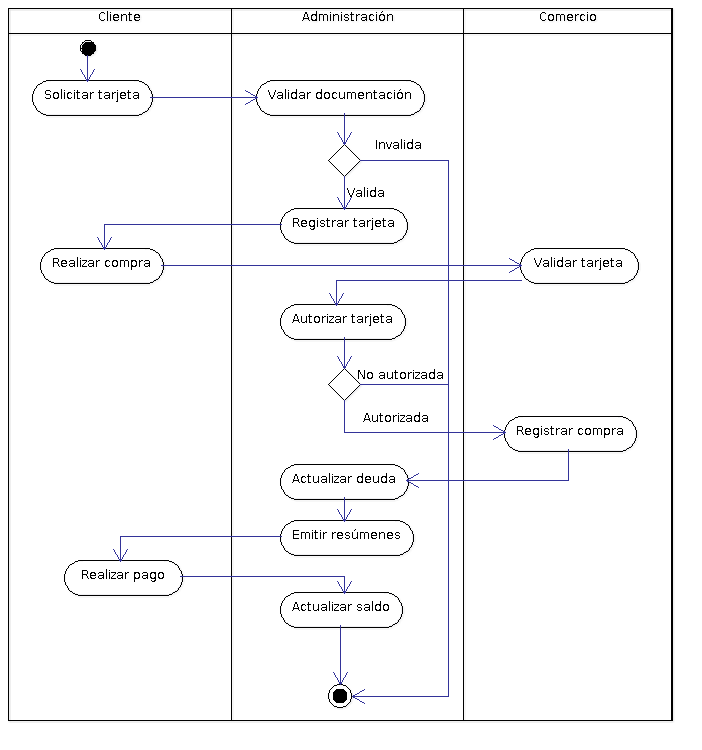
\includegraphics[width=0.9\textwidth]{images/mod_negocio_act_global.png}
\end{center}
\caption{Diagrama de actividades general de los procesos alcanzados por el
proyecto.}
\end{figure}

\begin{figure}[htb]
\begin{center}
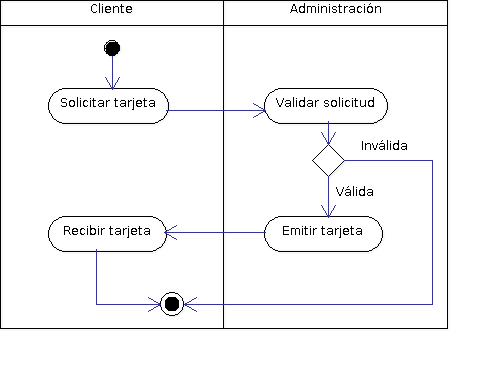
\includegraphics[width=0.7\textwidth]{images/mod_negocio_act_solicitudtarjeta.png}
\end{center}
\caption{Diagrama de actividades para el proceso de solicitud de una nueva
tarjeta.}
\end{figure}

\begin{figure}[htb]
\begin{center}
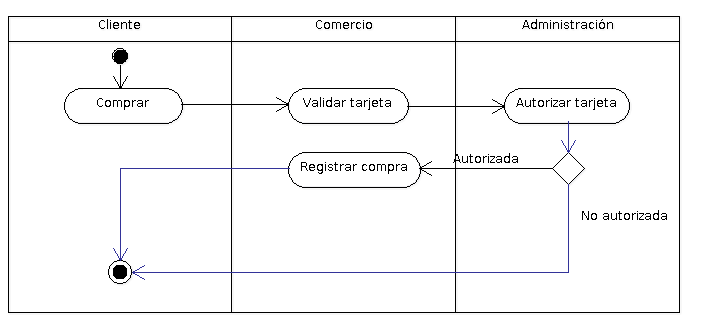
\includegraphics[width=0.9\textwidth]{images/mod_negocio_act_compra.png}
\end{center}
\caption{Diagrama de actividades para el proceso realización de una compra. El
comercio vende un producto y/o servicio a un cliente, quien opta por pagar por
este utilizando la tarjeta ShoppyCard.}
\end{figure}

\begin{figure}[htb]
\begin{center}
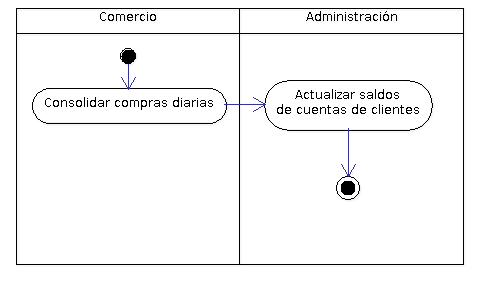
\includegraphics[width=0.7\textwidth]{images/mod_negocio_act_regcompras.png}
\end{center}
\caption{Diagrama de actividades para el proceso de actualización de saldos de
clientes. Diariamente, el comercio consolida la información de las compras
realizadas durante ese día y la envía a la administración.}
\end{figure}

\begin{figure}[htb]
\begin{center}
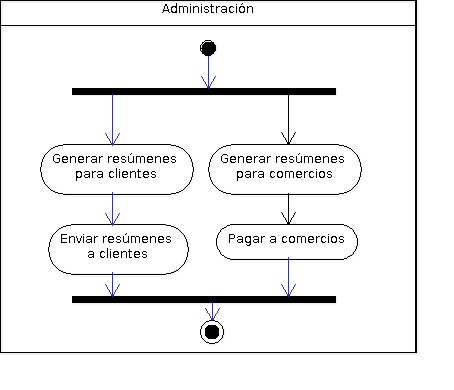
\includegraphics[width=0.7\textwidth]{images/mod_negocio_act_resumenes.png}
\end{center}
\caption{Diagrama de actividades para el proceso de emisión de resúmenes.
Mensualmente se generan los resúmenes de cuenta para los clientes, que son
enviados a cada cliente, y los resúmenes de saldo de cada comercio, utilizados
para realizar los pagos correspondientes.}
\end{figure}

\begin{figure}[htb]
\begin{center}
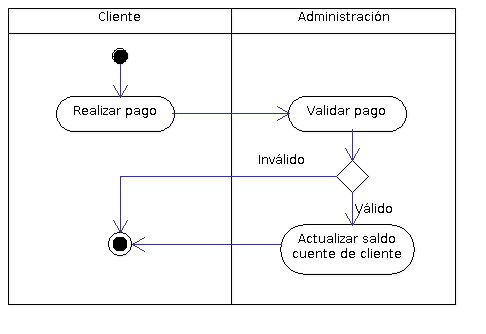
\includegraphics[width=0.7\textwidth]{images/mod_negocio_act_pago.png}
\end{center}
\caption{Diagrama de actividades para el proceso de pago. Del 1 al 10 de cada
mes, el cliente realiza el pago del importe detallado en el resumen que
recibió.}
\end{figure}

\FloatBarrier
